\section{Utility-based Selection Distillation}  
Unlike relevance emphasizes topical matching between query and passage, utility focuses on the usefulness in generating an answer, which is more important in RAG. 
However, directly using powerful LLMs to judge the utility of large-scale passages is computationally expensive. 
Moreover, ranking approach needs a threshold to determine the number of passages to generate an answer, which is not query-specific. 
Therefore, we propose a novel utility-based selection distillation approach. 
Specifically, utility-based distillation approach trains student selectors to learn pseudo-answer generation and utility judgment from teacher LLMs jointly. 
After distillation, the student model employs a front-to-back sliding window strategy to dynamically select optimal passage sets from large-scale candidates, which accounts for the dependency of pseudo-answers on input passages. 


\begin{figure}[h]
  \centering
  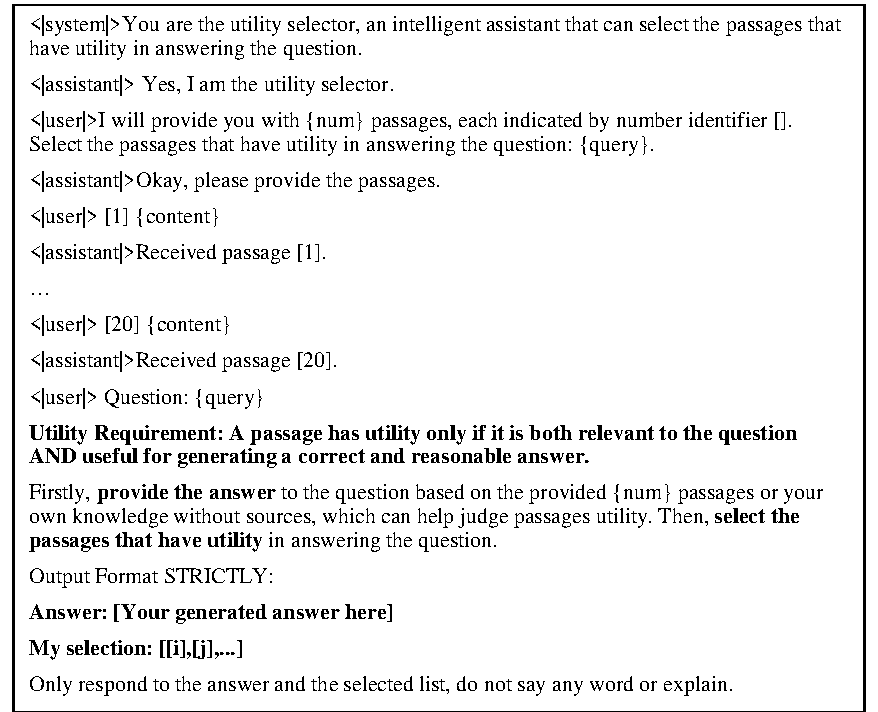
\includegraphics[width=\linewidth]{images/prompt.pdf}
  \caption{The prompt for utility-based selection. The bold is the special part for utility-based selection compared to relevance ranking.}
  \label{fig:prompt_utility}
\end{figure}

\subsection{Prompt Design} 
Figure \ref{fig:prompt_utility} shows the prompt utilized for utility-based selection. 
The relevance ranking prompt is the same as \citet{sun2023chatgpt}. 

\begin{figure*}[h]
  \centering
  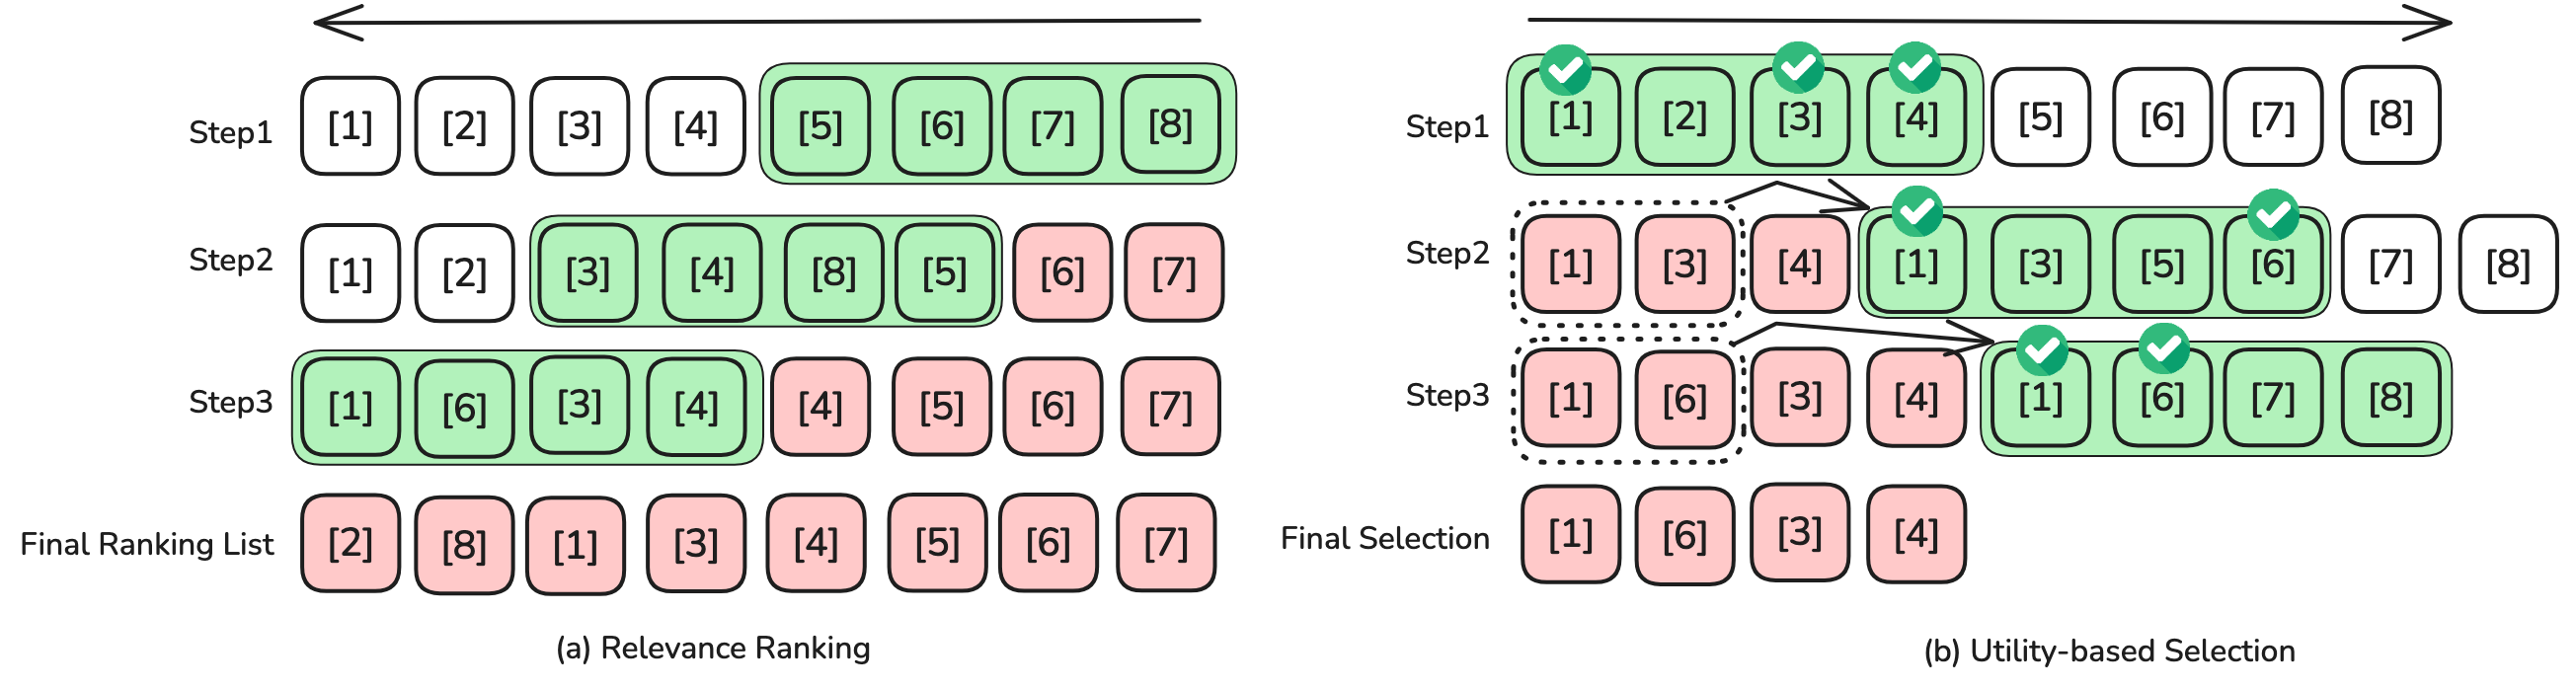
\includegraphics[width=\linewidth]{images/method.png}
  \caption{This diagram depicts an 8 passage selection ($M=8$) process using a sliding window $w=4$, stride $s=2$: (a) relevance ranking and (b) utility-based selection. Greed part means the windows, and the arrow indicates the direction of the window sliding. Passages shown in red are those that have undergone re-ranking or preselected passages. White passages denote unprocessed passages. For utility-based selection, $s$ documents (within the dashed-border box) from the preselected queue are placed into the processing window for utility-based selection. Documents selected within the current window are prepended to the head of the preselected queue.}
  \label{fig:sliding}
\end{figure*}
\subsection{Sliding Window for Utility-Based Selection} 
To overcome LLM token limitations during passage re-ranking, prior work often employs a sliding window strategy processed in back-to-front order \cite{sun2023chatgpt}, as shown in Figure \ref{fig:sliding} (a). This approach typically starts re-ranking the last $w$ passages (window size), then slides backwards by stride size $s$, re-ranking passages from position $(M-w-s)$ to $(M-s)$ and repeats until reaching the beginning of the list, where $M$ is the number of candidate passages. This back-to-front progression is effective for relevance permutation generation.

However, utility-based selection presents a distinct challenge: the generation of high-quality pseudo-answers, essential for estimating passage utility, is sensitive to the quality of the input passages provided to the LLM. 
Feeding lower-quality passages in the process can degrade pseudo-answer generation and subsequent utility judgments for all passages. 
To address this dependency and ensure robust pseudo-answer generation, we propose a forward-propagating sliding window strategy, processing passages from front to back.

As depicted in Figure \ref{fig:sliding} (b), our method operates as follows: 
For the first window (positions 1 to $w$), the LLM judges the utility of the $w$ passages within the current window and selects passages that have utility. 
Selected passages are prepended to the preselected queue. 
The original queue content is duplicated and positioned after the new selections.
The window slides forward by a stride size $s$. 
Specifically, the first $s$ passages from the current preselected queue are carried forward as input into the next window, which propagates high-utility context in the sequence. 
The next window now consists of these first $s$ propagated passages from the preselected queue, followed by the next $w-s$ unprocessed passages from the original list (maintaining their sequence). 
The LLM then performs utility-based selection within this new window context. Repeat until all $M$ passages have been processed. The final preselected queue represents the utility-based selection results.


